
\section*{SPATTs}
Solid Phase Adsorption Toxin Tracking (SPATTs) is new unique method of monitoring waterbodies. A Nitex mesh bag containing HP-20 resin (styrene-divinylbenzene copolymer) is submerged in waterbody of interest for a period of time. During this period, free-floating compounds will adsorb onto the polymer beads. SPATTs can are then retrieved and analyzed for chemical analytes of interest. This technique can be useful if sampling frequency is financially limited..





\section*{Methods}

A 1 meter x 5 centimeter strip of Nitex mesh were precisionaly cut. The Nitex strip was sewn by folding half lenth-wise (or \emph{hot dog} style). With tape holding the fold, the end of the strip was sewn 0.5cm from the edge. Stiching design was tight to ensure no leakage of polymer beads.

9-10cm of sewn Nitex strips were cut and zip-tied about 0.5cm at one end. 3.00-3.01 grams of HP-20 resin was filled using a funnel. The other end is zip-tied once the Nitex bag is full. SPATT bags are activated by soaking in 100\% methanol for 24 hours under $4^\circ$C. Next the SPATTs were rinsed with Milli-Q water and then soaked for 24 hours in Milli-Q water under $4^\circ$C before deploying the SPATTs bag in our target sample lakes.

At each lake site, two SPATT bags were loaded into a slotted PVC pipe. At each lake, a float was installed as described in section \ref{sampling}. SPATTs are left for about a month at each lake. When SPATTs are retrieved, they are carefully removed and rinsed with Milli-Q water and stored in a 15mL centrifuge vial with a plastic spacer on the bottom. SPATTs are stored at $4^\circ$ during transport back to the lab. The SPATTs are centrifuged at 8000rpm. The spacer allows liquid to pool on the bottom when centrifuged. When centrifuged, the SPATT bags are cut open and the resin is poured into a 50mL centrifuge tube. Milli-Q water is used to rinse the SPATT bags to effectivly transfer all the resin. About 30mL of Milli-Q water is used. The solution is allowed to rest so the resin settles to the bottom. Using a pipet, the water is carefully decanted until the total volume is 5mL.  A solution of 80\% methanol with 10$\mu$M ammonium formate is added to the tube until the total volume is 50mL. The solution is gently mixed and then allowed to settle for 30 minutes.

\section*{Results}

Out of all 12 congeners, MC-LA, MC-LR, and MC-RR were the most frequently detected congener.

\begin{table}[!ht]
\centering
  \caption*{Microcystin Congener from SPATTs}
  \label{}
\begin{tabular}{@{\extracolsep{5pt}}lccccc}
\\[-1.8ex]\hline
\hline \\[-1.8ex]
Statistic & \multicolumn{1}{c}{N} & \multicolumn{1}{c}{Mean} & \multicolumn{1}{c}{St. Dev.} & \multicolumn{1}{c}{Min} & \multicolumn{1}{c}{Max} \\
\hline \\[-1.8ex]
{[D-Asp3]}MC-RR & 91 & ND & ND & ND & ND \\
MC-RR & 91 & 164 & 1,116 & ND & 10,380 \\
Nodularin & 91 & 2 & 17 & ND & 160 \\
MC-YR & 91 & 10 & 30 & ND & 145 \\
MC-HtyR & 91 & 0 & 2 & ND & 18 \\
MC-LR & 91 & 353 & 1,211 & ND & 8,146 \\
{[D-Asp3]}MC-LR & 91 & 2 & 10 & ND & 92 \\
MC-HilR & 91 & 1 & 6 & ND & 53 \\
MC-WR & 91 & 0 & 1 & ND & 7 \\
MC-LA & 91 & 534 & 2,063 & ND & 13,977 \\
MC-LY & 91 & 1 & 11 & ND & 101 \\
MC-LW & 91 & 0 & 0 & ND & 0 \\
MC-LF & 91 & 0 & 2 & ND & 18 \\
Total MC & 91 & 1,066 & 3,273 & ND & 22,124 \\
\hline \\[-1.8ex]
\multicolumn{6}{r}{Values are expressed as (ng of MC / gram of resin)} \\
\end{tabular}
\end{table}

\begin{figure}[!ht]
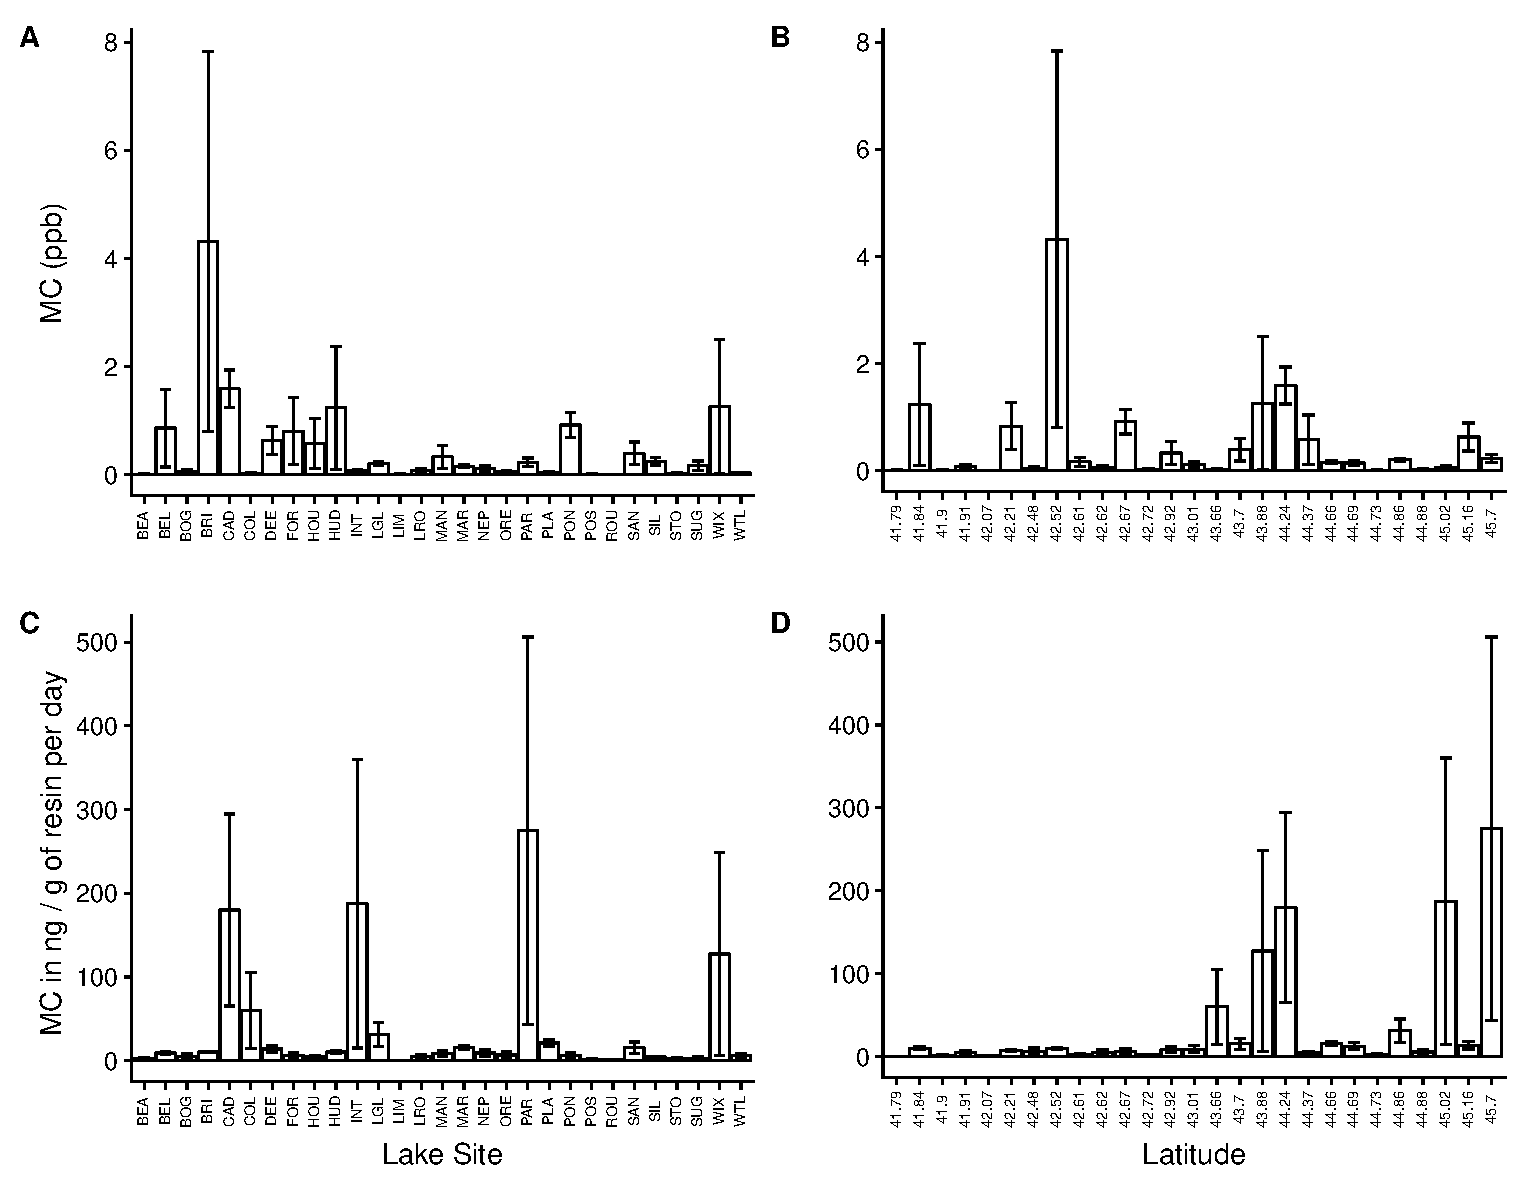
\includegraphics[width=\textwidth]{figures/spatttboxplotlake}
\label{spattbox}
\caption*{Comparitive Results of Microcystin Measured from SPATTS and Grab Samples}
A) B) C) D)
\end{figure}


\clearpage
\newpage
